\documentclass[12pt]{article}

\usepackage[english]{babel}
\usepackage[utf8x]{inputenc}
\usepackage{pdfpages}
\usepackage{lastpage} % Required to determine the last page for the footer
\usepackage{extramarks} % Required for headers and footers
\usepackage{graphicx} % Required to insert images
\usepackage{listings} % Required for insertion of code
\usepackage{courier} % Required for the courier font
\usepackage{hyperref} %hyperlink

% Margins
\topmargin=-0.45in
\evensidemargin=0in
\oddsidemargin=0in
\textwidth=6.5in
\textheight=9.0in
\headsep=0.25in

\linespread{1.1} % Line spacing

\newcommand{\Title}{Requirement Specification} % Assignment title
\newcommand{\Class}{Cos\ 301} % Course/class

\begin{document}

	\vspace{4em}
	
	\begin{center}%
	
	  \LARGE \bf \Title \\[4em]
	  \LARGE {\bf Group 2}\\[1em]
	  \LARGE {\bf Group Members:}\\[2em]
	  \large
	     Nico Taljaard					(10153285) \\[1em]
	     Abraham Daniel Pretorius		(12022404) \\[1em]
	     Mathys Ellis					(12019837) \\[1em]
	     Mbulungo Musetsho				(10176382) \\[1em]
	     Verushka Moodley				(29117454) \\[1em]
	     Eduan Bekker					(12214834) \\[1em]
	     Johan Esterhuyse				(10043285) \\[9em]
	     {\bf Version 3.0}
	    
	\end{center}
	
	\newpage
		{\LARGE \bf Change Log}\\[2em]
		
		\begin{tabbing}
			\hspace*{2.5cm}\=\hspace*{2.5cm}\=\hspace*{8cm}\=\hspace*{3cm} \kill
			10/02/2014	\> Version 1.0	\> Document Created 							\> Nico Taljaard \\
			15/02/2014	\> Version 1.0	\> System Description 							\> Mathys Ellis \\
			17/02/2014	\> Version 1.1	\> Edited Formatting 							\> Nico Taljaard \\
			17/02/2014	\> Version 1.1	\> Technical Specification 						\> Mbulungo Musetsho \\
			17/02/2014	\> Version 1.1	\> Created Non-functional Requirements 			\> Eduan Bekker \\
			18/02/2014	\> Version 1.2	\> External Interface Requirements 				\> Abraham Daniel Pretorius  \\
			18/02/2014	\> Version 1.2	\> Functional Requirement 						\> Nico Taljaard \\
			18/02/2014	\> Version 1.2	\> Updated Non-functional Requirements 			\> Eduan Bekker \\
			18/02/2014	\> Version 1.2	\> Updated External Interface Requirements 		\> Abraham Daniel Pretorius  \\
			18/02/2014	\> Version 1.2	\> Updated System Description 					\> Mathys Ellis \\
			20/02/2014	\> Version 1.3	\> Introduction 								\> Verushka Moodley \\
			20/02/2014	\> Version 1.3	\> Fixed Compile Errors 						\> Nico Taljaard \\
			20/02/2014	\> Version 1.2	\> Updated External Interface Requirements 		\> Abraham Daniel Pretorius  \\
			21/02/2014	\> Version 1.2	\> Fixed Spelling 								\> Nico Taljaard \\
			21/02/2014	\> Version 2.0	\> Change formatting 							\> Nico Taljaard \\
			23/02/2014	\> Version 2.0	\> Checked spelling and grammar 				\> Mathys Ellis \\
			24/02/2014	\> Version 3.0	\> Changed to new layout specification 			\> Nico Taljaard \\
			24/02/2014	\> Version 3.0	\> Required Functionality 						\> Nico Taljaard \\
			24/02/2014	\> Version 3.0	\> Quality requirements 						\> Eduan Bekker \\
			24/02/2014	\> Version 3.0	\> Integration Requirements						\> Abraham Daniel Pretorius \\
			26/02/2014	\> Version 3.0 	\> Use Cases									\> Johan Esterhuyse \\	
			26/02/2014	\> Version 3.0 	\> Appended Integration Requirements			\> Abraham Daniel Pretorius \\
			27/02/2014	\> Version 3.0	\> Added use case prioritization and added		\> \\
						\>				\> possible glossary terms with out definitions	\> Mathys Ellis \\
			27/02/2014	\> Version 3.0	\> Domain Objects								\> Abraham Daniel Pretorius \\
			27/02/2014	\> Version 3.0	\> Domain Objects								\> Eduan Bekker \\
						\>				\>												\> Mbulungo Musetsho \\
			27/02/2014	\> Version 3.0	\> Appended architecture requirements			\> Nico Taljaard \\
			27/02/2014	\> Version 3.0	\> Scope and Limitations/Exclusions				\> Nico Taljaard \\
			27/02/2014	\> Version 3.0	\> Glossary and document unification			\> Nico Taljaard \\
			27/02/2014	\> Version 3.0	\> Final formatting changes						\> Nico Taljaard \\
		\end{tabbing}

	\newpage
	\tableofcontents
	
	\vspace{0.5in}
	
	\begin{flushleft}
		\LARGE\href{https://github.com/njTaljaard/Cos301_Phase1/}{GitHub repository: Mini project - Phase 1 -  Group 2}
	\end{flushleft}
	
	\newpage
	\section{Introduction}
	
		\vspace{0.2in}
	
		This document is the software requirements specification for a computerised marking system to be used by the University of Pretoria. It begins by addressing the purpose and vision of the project then continues with a general discussion on the background of the project. Thereafter, the architectural requirements are identified with a main focus on the access channel requirements, quality requirements, integration requirements, and architectural constraints. The function requirements follow by discussing the application functionality required by the users of the system.  In this section of the document, many diagrams are used to depict the flow of communication and interaction between the users and the system. It will also illustrate the processes that the system will need to complete and the states that the system will under go.  The next topic will communicate the open issues on some of the requirements, and the document concludes with a glossary of possibly unfamiliar terms used in this document.
		
	\section{Vision}
	
		\vspace{0.2in}
		
		The purpose of this document is to communicate the requirements and proposed solution to the client, Mr Jan Kroeze, who requires a computer system for marking purposes. This document will outline the scope of the project and thus serve as a formal agreement and contract between the developers and the client. It will also serve as a reference and eliminate any confusion that may occur in the later stages of development.
	
	\section{Background}

		\vspace{0.2in}
		The University of Pretoria currently has a manual paper based marking system which has many flaws such as: losing marks is one of the major issues. Our solution aims to assist them by providing a computerised system. The required computer system should aid the marker and lecturers at the university in recording marks of assessments for students, and the maintenance of marks thereafter. It should also allow students to keep track with their marks.
		
		\vspace{0.1in}
		
		\begin{flushleft}
			The solution will consist of an application that students, markers and lecturers will use in the following way:
		\end{flushleft}
		
		\begin{itemize}
			\item Markers will receive mark list of students and will be allowed to assign practical marks to the students via the mobile application. Lecturers will also be granted these permissions.
			\item Students will be able to view a list of their marks via the application
		\end{itemize}
		
		\vspace{0.1in}
		
		\begin{flushleft}
			The solution will also consist of a web interface that will allow the following:
		\end{flushleft}
		
		\begin{itemize}
			\item Lecturers can maintain and integrate marks
			\item Lecturers can request reports with a certain criteria. A graph of some nature or statistics will then be presented 
			\item An audit log will be updated automatically 
		\end{itemize}
		
		\vspace{0.1in}
		
		\begin{flushleft}
			The solution has the following restrictions:
		\end{flushleft}
		
		\begin{itemize}
			\item Users must be registered - A username and password is required for access to the system
			\item Marking lists may only be locked/unlocked by lecturers that are assigned to the course. Markers will be allowed to update marks according to the status of the mark list. Students may only view their mark when the mark list is locked.
			\item No one may be allowed to edit the audit log. Only lecturers have permission to view the audit log. 
		\end{itemize}

		\vspace{0.2in}

	\section{Architecture requirements}
	
		\vspace{0.2in}
		
		\subsection{Access channel requirements}
		
			\vspace{0.2in}
			\begin{itemize}
				\item Marker will gain access the mobile android application as well as the web interface can be used.
				\item Lectures have to use the web interface to administrate their modules and view audit logs.
				\item Student view all allocated marks through the mobile application as well as the web interface.
				\item Administrators use the web interface to view audits and control all lectures and modules.
			\end{itemize}
			

		\subsection{Quality requirements}
		
			\vspace{0.2in}
			
			\begin{itemize}
			
				\item Authentication
					\begin{itemize}
						\item All users have to login before they are able to access the system using a user name to identify, a password to authenticate where upon the authorized permissions will be granted.
					\end{itemize}
				
				\item Audit-ability
					\begin{itemize}
						\item All the actions of all the users will be added to the audit log.
						\item The events consider as audit trails will include:
						
						\begin{itemize}
							\item The login and logout of users.
							\item The assignment of marks.
							\item The modifications of any data.
						\end{itemize}	
					\end{itemize}

				\item Scalability
					\begin{itemize}
						\item The system should be able to handle multiple running practicals simultaneously
						\item The performance of the system should not be dependent on the number of concurrent users
					\end{itemize}
				
				\item Availability
				
					\begin{flushleft}
						The system should be available 99\% of the time if the under the pre-condition that the correct authentication information has been provided.
					\end{flushleft}
					
			\end{itemize}

		\subsection{Integration requirements}
		
		\vspace{0.2in}

		\begin{flushleft}
			\textbf{Integration channel to be used:}
			\newline\textbf{(Priority: High, Requirement: ARQIRQ1)} 
		\end{flushleft}

			\vspace{0.05in} 
			\begin{itemize} 
				\item SOAP will be used as an interface\
				 between different mediums and platforms to interact with the system.
			\end{itemize} 

			\vspace{0.15in}

		\newpage
		
		\begin{flushleft}
				\textbf{Protocols}
				\newline\textbf{(Priority: High, Requirement: ARQIRQ2)} 
		\end{flushleft}
			
			\vspace{0.05in} 

			\begin{itemize}
				\item SOAP will be used to pull reports of marks and audit logs using XML formatting.
				\item LDAP will enable the SSO ability of the system.
			\end{itemize}

			\vspace{0.15in}

		\begin{flushleft}
			\textbf{API specifications}
			\newline\textbf{(Priority: High, Requirement: ARQIRQ3)}
		\end{flushleft}
		
			\vspace{0.05in}
			
			The system has to interface with the following mediums:
			\begin{itemize}
				\item Internal API for Android application.
				\item External API for data transfer between interconnecting systems. This API uses SOAP
				transfer the data.
			\end{itemize}
			
			\vspace{0.05in} 
		
		All API's should represent their data from SOAP to:
		\begin{itemize}
			\item XML for interfacing with web servers using WSDL.
			\item Output marks to .CSV format.
		\end{itemize}
	
	\vspace{0.15in}

	\begin{flushleft}
		\textbf{Quality requirements for integration}
		\newline\textbf{(Priority: High, Requirement: ARQIRQ4)}
	\end{flushleft}

		
	\vspace{0.05in}
			
	\begin{itemize}
		\item Performance:
		\begin{itemize}
			\item 	People viewing the marks should not need to wait extensively, //
		 			however the system can only be as fast as the connection to it.//
		 			There for the system cannot be expected to be faster than the connection\\
		 			that is being used.
			\item Documentation drawn up from the marks may take between  \\
					10 - 30 seconds to be compiled.
			\item Markers should be able to update marks within 10 seconds of each other.
		\end{itemize}
		
		\item Scalability:
		\begin{itemize}
			\item The system will be designed with design patterns. These are used so that\\
			the it is easy to upgrade the different aspects independently. \\   
		\end{itemize}

		\item Reliability:
		\begin{itemize}
			\item A software issue should not arise, but if it does the application \\
			must handle the problem and send an appropriate error message to the user. \\
			If data has failed to send the application must reattempt to upload the data \\
			for a specified amount of time (1 minute) or until such a time that the user \\
			aborts data transfer.		
		\end{itemize}
			
			
		\item Security:
				\begin{itemize}
				\item No user, who is unauthorized, may gain access to the system.
				\item Authorized users can only access the aspects of the system as \\
				allocated to them by the administrator.
				\item Security questions, as well as email addresses will be linked to each\\
					of the users. This will be used for password recovery.
				\end{itemize}
				
				
		\item Auditability:
				\begin{itemize}
				\item Each time marks are changed it will be recorded in an audit trail which not\\
				even the system administrator would be able to edit.
				\end{itemize}
				
	\end{itemize}
			
	\vspace{0.2in}
			
	\subsection{Architecture constraints}
	
		\vspace{0.2in}
		
		\begin{flushleft}
			\textbf{Technologies which MUST be used}
			\newline\textbf{(Priority: High, Requirement: ARQ1)}
		\end{flushleft}
			
		\vspace{0.05in}
		\begin{itemize}
			\item The system must support the following platforms: 
			\begin{itemize}
				\item Android (API 15)
				\item Web browser (with HTML 5 compatibility)
			\end{itemize}
				
			\item The system must strictly operate over HTTPS
			\item The following technologies and languages must be used for implementation purposes:
			\begin{itemize}
				\item Python with Django (server-side programming)
				\item Java ( Android Module Development)
				\item MySQL (Database)
			\end{itemize}
			\item SOAP interface must be utilized for this system
			\item LDAP (account management)
		\end{itemize}
		
		
	
	\section{Functional requirements}
	
		\vspace{0.2in}
		
		\subsection{Introduction}
			\begin{flushleft}
				\vspace{0.2in}
	
				The goal of the system is to provide the client with a secure, scalable and remotely accessible marking and mark management system. The system is comprised of four different facets which are listed below. It is intended to replace the current marking and mark management system employed by the client, which is currently paper and spreadsheet based.
				
				\vspace{0.5cm}
				\textbf{Student mark retrieval facet:}
				\vspace{0.1in}
				\\
				The goal of this facet is to provide the "Students" with a secure and private means to a read-only view of their marks, for the markable items of a specified course on the system. The means by which they will view the markable items will be in the form of a web interface and android application.
				
				\vspace{0.5cm}
				\textbf{Marker marking tool facet:}
				\vspace{0.1in}
				\\
				The goal of this facet is to provide "Markers", assigned to a particular course, with a mobile application to allow then to be able to add and update the mark of a specified student on the mark list for a particular markable item of the particular course. The application will allow "Markers" access to the mark list from any location where an internet connection is available. The application will be in the forms of a website interface and android application.
				
				\vspace{0.5cm}
				\textbf{Lecturer mark management facet:}
				\vspace{0.1in}
				\\
				The goal of this facet is to provide "Lectures", assigned to a particular course, with a means to manage the marks of each student registered to the course and mark structure of the course. Where the term manage comprises of adding, modifying and removing markable items, mark lists and the individual marks of students. Further the facet also has the goal of providing a means to report on mark related data on different levels of granularity of a particular course.
				
				\vspace{0.5cm}
				\textbf{Audit trail facet:}
				\vspace{0.1in}
				\\
				The goal of this facet is to give the system the ability to track all critical actions that occur on the system independent of any user interference and also provide a read-only view of such trails for authorised users of the system. Where critical actions comprise of adding, updating and removing any data on the database as well as login and logout actions.
			\end{flushleft}
			
			
			\vspace{0.2in}
			
		\subsection{Scope and Limitations/Exclusions}
		
			\vspace{0.2in}
			
			\begin{flushleft}
				\textbf{Scope:}
			\end{flushleft}
			
			The scope is fully depicted through the entire document.
			
			\begin{flushleft}
				\textbf{Limitations}
			\end{flushleft}
						
			\vspace{0.02in}
			
			\begin{itemize}
				\item This system should not integrate with the "existing marking system" of the university. It will only be tested within one 
				\item Authentication is verified through an external system and not part of this system specification.
			\end{itemize}
			
			
		\vspace{0.2in}
		
		\subsection{Required functionality}
		
			\vspace{0.2in}
			
			\begin{flushleft}
				\textbf{Course API}
				\newline\textbf{(Priority: High, Requirement: FRQ1)}
			\end{flushleft}
			
			\vspace{0.02in}
			
				\begin{itemize}
					\item A course must be creatable.
					\item Lectures must be added to course by users with correct authorization.
					\item Lectures must be able to add markers to the course, as well as be able to assign them to a practical time slot.
					\item Student information for each student that is assigned to a practical time slot of a course should be pulled from an existing database so that teaching assistants and tutors of the course can find the student to be marked.
				\end{itemize}
				
			\vspace{0.15in}
				
			\begin{flushleft}
				\textbf{Lecturer API}
				\newline\textbf{(Priority: High, Requirement: FRQ2)}
			\end{flushleft}
						
			\vspace{0.02in}
			
			\begin{itemize}
				\item A tasks must be creatable for the following:
						\begin{itemize}
							\item Practicals
							\item Assignments
							\item Class tests
							\item Tests
						\end{itemize}
				\item Tasks should also contain the following information:
						\begin{itemize}
							\item Starting time to open access.
							\item End time if a specified time is required, else manual locking is required by lecture.
							\item A rubric must be added to show the mark allocation.
						\end{itemize}
				\item Adjust mark weight allocations.
				\item Lectures alone should be able to change marks of his own subjects.
				\item Assign security roles to markers.
				\item Move students to a different markers.
				\item Use the reporting API.
			\end{itemize}
				
			\vspace{0.15in}
			
			\begin{flushleft}	
				\textbf{Auditing API}
				\textbf{(Priority: High, Requirement: FRQ3)}
			\end{flushleft}
			
			\vspace{0.02in}
			
			\begin{itemize}
				\item Log file for following activities:
				\begin{itemize}
				 	\item Marks added by whom and when.
				 	\item Marks changed or removed by who, when and what is the reason.
				 	\item Login and logout activities
				\end{itemize}
	
				\item Lectures must be able view only the audit logs of the course(s) they are assigned to.
				\item Head of Department alone should assign a user that can view the entire change log.
				\item No edits to the audit log allowed.
			\end{itemize}
				
			\vspace{0.15in}
				
			\begin{flushleft}
				\textbf{Marking API}
				\textbf{(Priority: High, Requirement: FRQ4)}
			\end{flushleft}
						
			\vspace{0.02in}
			
			\begin{itemize}
				\item Accessible through mobile application for markers.
				\item Display all available mark lists for markers to mark.
				\item Within mark list display all students registered for current session with a search option.
				\item Search filters should be available for student number, surname or name. The displayed results should contain all the results that match the filters.
				\item For the selected student the marking rubric should be displayed with type able fields.
				\item Marks should be submitted to the database directly after mark has been finalized for each student.
			\end{itemize}
				
			\vspace{0.15in}
			
			\begin{flushleft}
				\textbf{Reports API}
				\textbf{(Priority: Medium-High, Requirement: FRQ5)}
			\end{flushleft}
						
			\vspace{0.02in}
			
			\begin{itemize}
				\item Marks can be exported in a .csv file containing the selected marks for each student.
				\item All reports should be based on a select set of marks.
				\item Numeric statistics can be exported about marks.
				\item Graphical reports should be exported to .pdf file.
			\end{itemize}
				
			\vspace{0.2in}
			
			\begin{flushleft}
				\textbf{Student API}
				\textbf{(Priority: Medium, Requirement: FRQ6)}
			\end{flushleft}
			
			\vspace{0.02in}
			
			\begin{itemize}
				\item Accessible through mobile application or web interface.
				\item Landing page displays all courses of current student.
				\item Course marks should be viewable for separate assessments as well as a progress mark of a particular course.
			\end{itemize}
				
			\vspace{0.2in}
		
		\subsection{Use case prioritization}
		
			\vspace{0.2in}
			
			\begin{itemize}
				\item \textbf{Critical:}
					\begin{itemize}
						\item Log in [1.1; 2.1; 3.1; 4.1]
						\item Create assessment [1.10]
						\item Set rubric [1.12]
						\item Set constraints [1.13]
						\item Set markers [1.14]
						\item Select assessment [1.11; 2.3; 3.5]
						\item Mark assessment [2.5]
						\item Submit marks [2.6]
						\item Select course [1.2; 2.2; 3.2; 4.2]						
						\item Select student [1.6; 2.4]	
						\item View marks [3.3]
						\item View overall marks [1.3]					
						\item Export marks [1.4]
						\item View entire audit trail [4.4]
					\end{itemize}
				\item \textbf{Important:}
					\begin{itemize}
						\item View student marks [1.5]
						\item View students overall marks [1.8]						
						\item Update assessment [1.9]
						\item Update rubric
						\item Update markers
						\item Update constraints
						\item View assessment mark [3.4]
					\end{itemize}
				\item \textbf{Nice-to-Have:}
					\begin{itemize}
						\item Export entire audit trail [4.4]
						\item Select user [4.5]
						\item View individual audit trail [4.3]
						\item Export user audit trail
					\end{itemize}
			\end{itemize}
			
		\newpage
		\vspace{0.2in}
		
		\subsection{Use case/Services contracts}
		
			\vspace{0.2in}
			
			\begin{figure}[http]
				\centering
				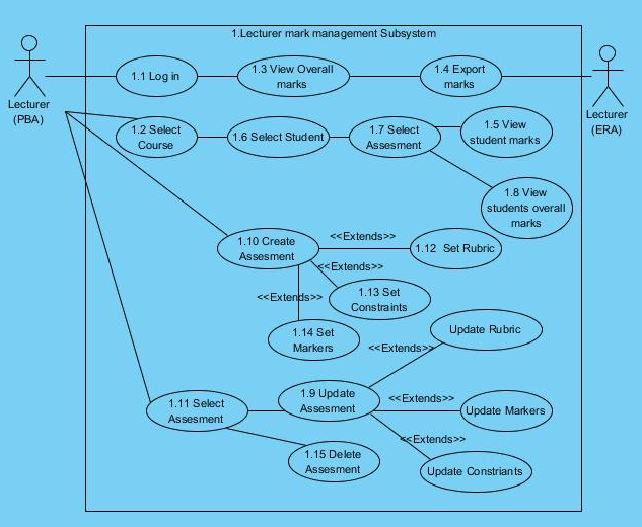
\includegraphics[width=7in, height=5in]{./UML/LectureAPI.jpg}
			\end{figure}
			
			\begin{figure}[http]
				\centering
				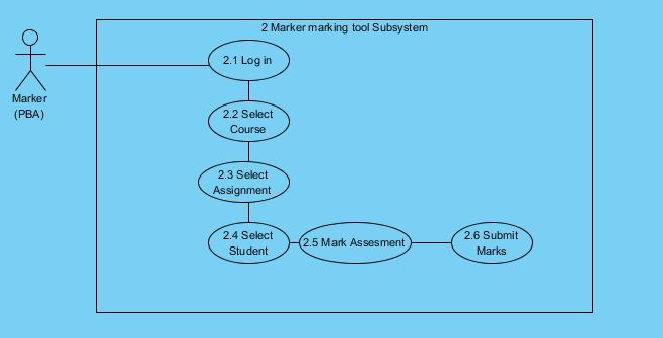
\includegraphics[width=6in, height=4in]{./UML/MarkerAPI.jpg}
			\end{figure}
			
			\begin{figure}[http]
				\centering
				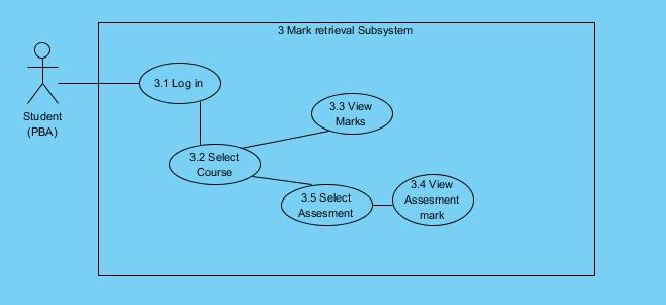
\includegraphics[width=6in, height=4in]{./UML/MarkRetrieval.jpg}
			\end{figure}
			
			\begin{figure}[http]
				\centering
				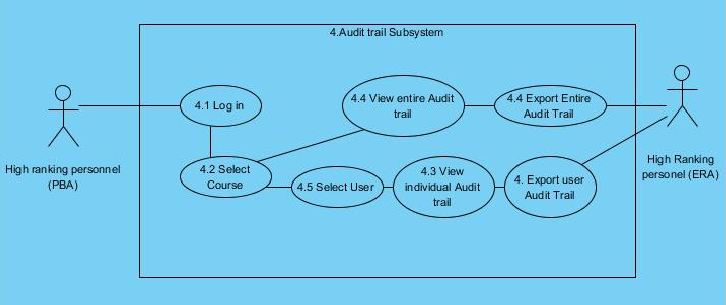
\includegraphics[width=6in, height=3in]{./UML/AuditAPI.jpg}
			\end{figure}
			
		\newpage
		\vspace{0.2in}
						
		\subsection{Process specifications}
		
			\vspace{0.2in}
			
			\begin{figure}[http]
				\centering
				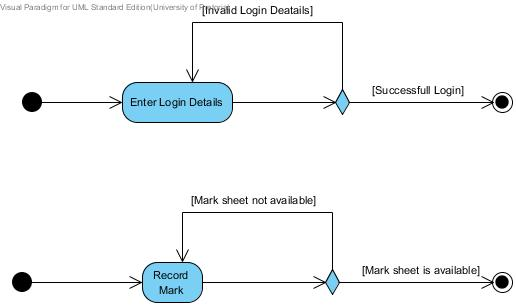
\includegraphics[width=3.5in, height=3.5in]{./UML/ProcessSpecifications.jpg}
			\end{figure}
		
		\newpage
		\vspace{0.2in}
		
		\subsection{Domain Objects}
		
			\vspace{0.2in}
			
			\begin{figure}[http]
				\centering
				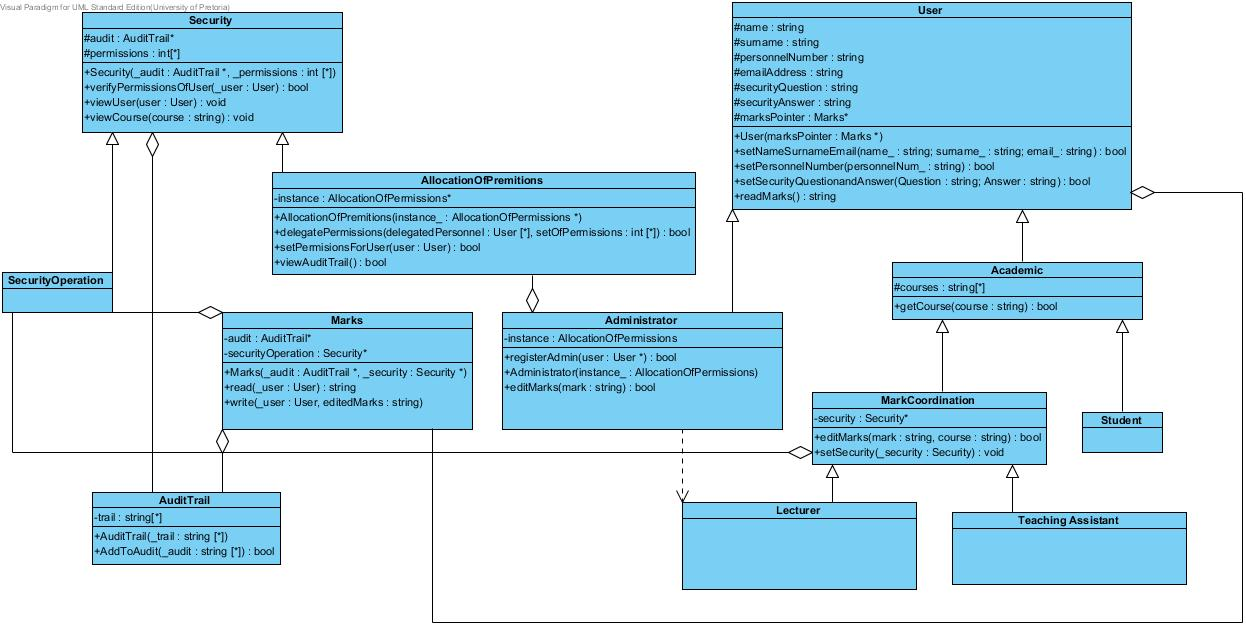
\includegraphics[width=7in, height=6in]{./UML/DomainObjects.jpg}
			\end{figure}
	
		\newpage
		\vspace{0.2in}
		
	\section{Open Issues}
	
		\vspace{0.2in}
		
	\section{Glossary}
	
		\vspace{0.2in}
		\begin{itemize}
			\item Student - Entailing all students register at the university for specific modules.
			\item Marker - A grouping of including Teaching Assistance and Tutors, which have permission to assign marks.
			\item Lecturer - Co-ordinator and/or module presenter.
			
			\item Markable item - Including tests, class tests, assignments, practicals.
			\item Mark list - List consisting of all students registered for a specific module.
			\item Course - A module presented at the university.
			
			\item Web interface - Browser client.
			\item SSO - Single Sign On.
			\item LDAP - System used during SSO for authentication.
			\item SOAP - Simple Object Access Protocol.
			\item API -	A sub-section of the overall system.
			\item HTTPS - Secured HTTP connection.
			\item HTML 5 - Standardised version of HTML.
			\item PDF -	The format used in statistics exports.
			\item CSV -	Column Separated Values, used for import of marks and student information.
			\item SOAP - Simple Object Access Protocol	
			\item WSDL - Web Service Definition Language
			\item Android - Mobile operating system used.
			\item Django - Web framework used for the systems back-end.
			\item Python - Programming language used in Django.
			\item Java - Used by Android to program application.
			\item MySQL - Language for database structure and queries.
		\end{itemize}	
	
\end{document}
